\documentclass[11pt]{article}
\usepackage{algorithm2e}
\usepackage[bottom]{footmisc} 
\usepackage[italian]{babel}
\usepackage[document]{ragged2e}
\justifying
\usepackage{amsfonts, amssymb, amsmath}
\usepackage{cancel}
\usepackage{float}
\usepackage{mathtools}
\usepackage[margin=3cm]{geometry}
% \setcounter{secnumdepth}{0}
\usepackage{hyperref}
\hypersetup{
    colorlinks,
    citecolor=black,
    filecolor=black,
    linkcolor=black,
    urlcolor=black
}
\usepackage{array}
\usepackage{makecell}
\usepackage{tikz}
\usetikzlibrary{arrows, positioning, quotes, shapes.geometric}
\usepackage{hyperref}
\usepackage[noabbrev,capitalize,italian]{cleveref}
\newcommand{\fref}[1]{\hyperref[#1]{\cref{#1}}}
\usepackage{makecell}
\usepackage{etoolbox}
\patchcmd{\thebibliography}{\section*{\refname}}{}{}{}
\usepackage{enumitem}

\tolerance=1
\emergencystretch=\maxdimen
\hyphenpenalty=10000
\hbadness=10000



% --- MACRO ---

% Box user story
% {US}{Punti}{DoD}{Test}{Epica}
\newcommand{\userstory}[5]{%
    \begin{center}
    \fbox{\parbox{15cm}{%
        \begin{minipage}{9.8cm}
            \textbf{US}: #1\\
            \textbf{Epica}: #5
        \end{minipage}
        \hfill
        \begin{minipage}{5cm}
            \begin{flushright}
                \textbf{Punti}: #2
            \end{flushright}
        \end{minipage}
        \vspace*{6pt}

        \textbf{DOD}: #3\\

        \def\temp{#4}\ifx\temp\empty
            %
        \else
            \textbf{Test}: #4\\
        \fi
    }}
    \end{center}
}

% {Nome}{Responsabilità}{Collaborazioni}
\newcommand{\crc}[3]{%
    \begin{center}
        \fbox{\parbox{15cm}{%
            \vspace*{0.3em}

            \begin{minipage}{13cm}
                \textbf{Nome}: \texttt{#1}\\
            \end{minipage}
            \vspace*{0.5em}

            \begin{minipage}[t]{0.45\textwidth}
                \textbf{Responsabilità}
                \def\temp{#2}\ifx\temp\empty
                    %
                \else
                    \begin{itemize}[topsep=0.2em]
                        \setlength\itemsep{-0.5em}
                        #2
                    \end{itemize}
                \fi
            \end{minipage}
            \hfill\vline\hfill
            \begin{minipage}[t]{0.45\textwidth}
                \textbf{Collaborazioni}
                \def\temp{#3}\ifx\temp\empty
                    %
                \else
                    \begin{itemize}[topsep=0.2em]
                        \setlength\itemsep{-0.5em}
                        #3
                    \end{itemize}
                \fi
            \end{minipage}
            
            \vspace*{0.3em}
        }}
    \end{center}
}



\begin{document}
\begin{titlepage}
    \begin{center}
        \vspace*{1.5cm}
            
        \Huge
        \textbf{Rapporto del TEAM 12}
            
        \vspace{0.3cm}
        \LARGE
        Tweet Analysis\\[0.2em]

        \vspace{1.5cm}
          
        \begin{minipage}[t]{0.47\textwidth}
            \begin{center}
                \parbox{50mm}{\centering\large {\bf Cheikh Ibrahim $\cdot$ Zaid} \\[0.2em] PO Operativo \\[0.3em] Matricola: \texttt{0000974909}}\\[2em]
                \parbox{50mm}{\centering\large {\bf Lee $\cdot$ Qun Hao Henry} \\[0.2em] Developer \\[0.3em] Matricola: \texttt{0000990259}}
            \end{center}
		\end{minipage}
		\hfill
		\begin{minipage}[t]{0.47\textwidth}\raggedleft
            \begin{center}
                \parbox{50mm}{\centering\large {\bf Xia $\cdot$ Tian Cheng} \\[0.2em] Scrum master \\[0.3em] Matricola: \texttt{0000975129}}\\[2em]
                \parbox{50mm}{\centering\large {\bf Paris $\cdot$ Manuel} \\[0.2em] Developer \\[0.3em] Matricola: \texttt{0000997526}}
            \end{center}
		\end{minipage}  
            
        \vspace{6cm}
            
        Anno accademico\\
        $2022 - 2023$
            
        \vspace{0.8cm}
            
            
        \Large
        Corso di Ingegneria del Software\\
        Alma Mater Studiorum $\cdot$ Università di Bologna\\
            
    \end{center}
\end{titlepage}
\pagebreak


\tableofcontents
\newpage


\section{Descrizione del prodotto}
\subsection{Scope}
Il prodotto realizzato è un client Twitter in grado di fornire analisi e funzionalità specifiche per determinate tematiche.\\
In particolare sono state richieste le seguenti funzioni:
\begin{itemize}
    \item Ricerca e visualizzazione di tweet con filtri di ricerca, grafici per l'analisi aggregata e mappa per la geolocalizzazione.
    \item Partita a scacchi contro gli utenti di Twitter che giocano la propria mossa a maggioranza.
    \item Raccolta dei tweet degli spettatori dei giochi televisivi \textit{L'Eredità} e \textit{Reazione a Catena}, visualizzando i tentativi e i vincitori.
    \item Visualizzazione di una sintesi dei punteggi, di statistiche e delle squadre partecipanti degli altri utenti riguardanti il \textit{Fantacitorio}.
\end{itemize}

Il backlog è stato partizionato in cinque epiche:
\begin{center}
    \begin{tabular}{ | m{8em} | m{11cm} | }
        \hline
        {\textbf{Epica}} & {\textbf{Descrizione}} \\
        \hline
        Raccolta e analisi di tweet & Prime funzionalità per ricercare e analizzare tweet \\ 
        \hline
        Scacchi & Partita a scacchi contro gli utenti di Twitter che scelgono a maggioranza la mossa \\ 
        \hline
        L'Eredità & Raccolta dei tentativi degli utenti di Twitter di indovinare la \textit{Ghigliottina} \\ 
        \hline
        Reazione a catena & Raccolta dei tentativi degli utenti di Twitter di indovinare la \textit{Catena Finale} \\ 
        \hline
        Fantacitorio & Raccolta e visualizzazione dei punteggi del Fantacitorio e ricerca delle squadre degli altri utenti \\ 
        \hline
    \end{tabular}
\end{center}
Le user stories contenute in ciascuna epica sono descritte nella \fref{sprint_description}.\\~\\

Il prodotto è attivo online \cite{deploy_prod}, assieme ad un video dimostrativo \cite{video}.


\subsection{Casi d'uso}
\begin{figure}[H]
    \centering
    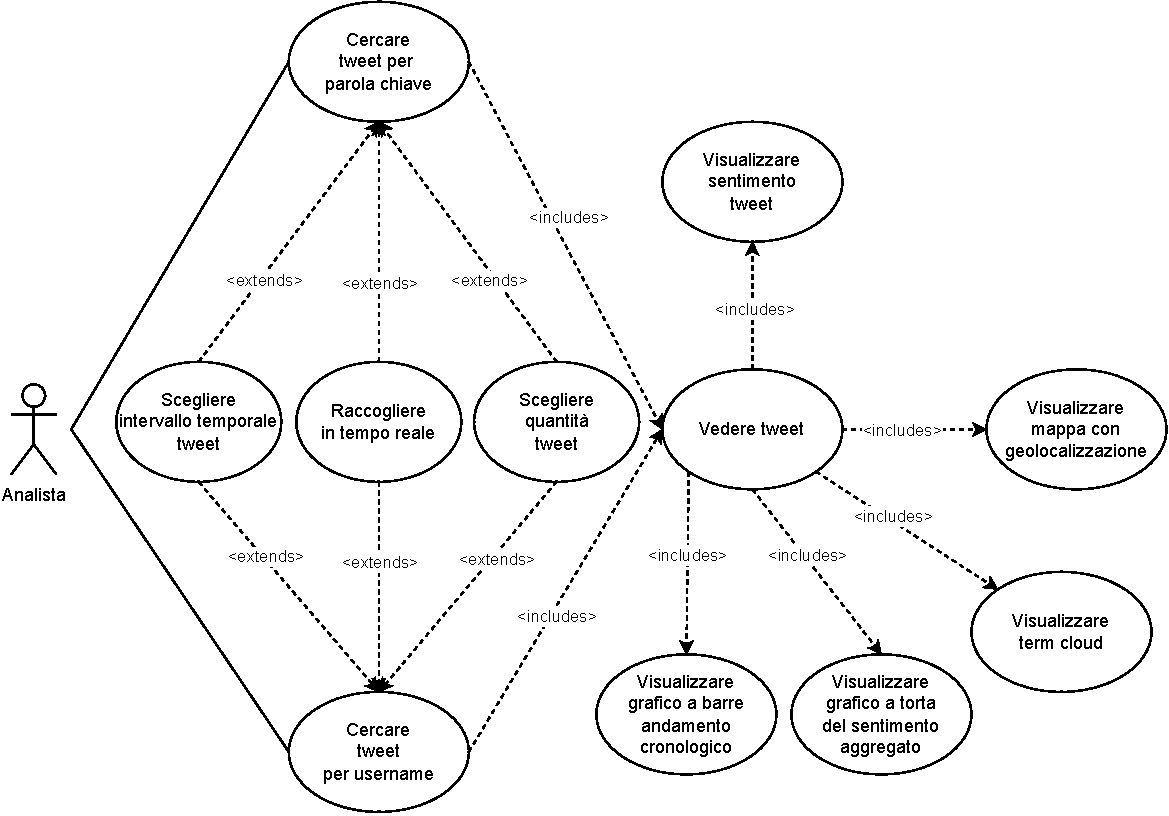
\includegraphics[scale=0.7]{./img/usecase/tweet.pdf}
    \caption{Casi d'uso per l'epica: Raccolta e analisi di tweet}
\end{figure}

\begin{figure}[H]
    \centering
    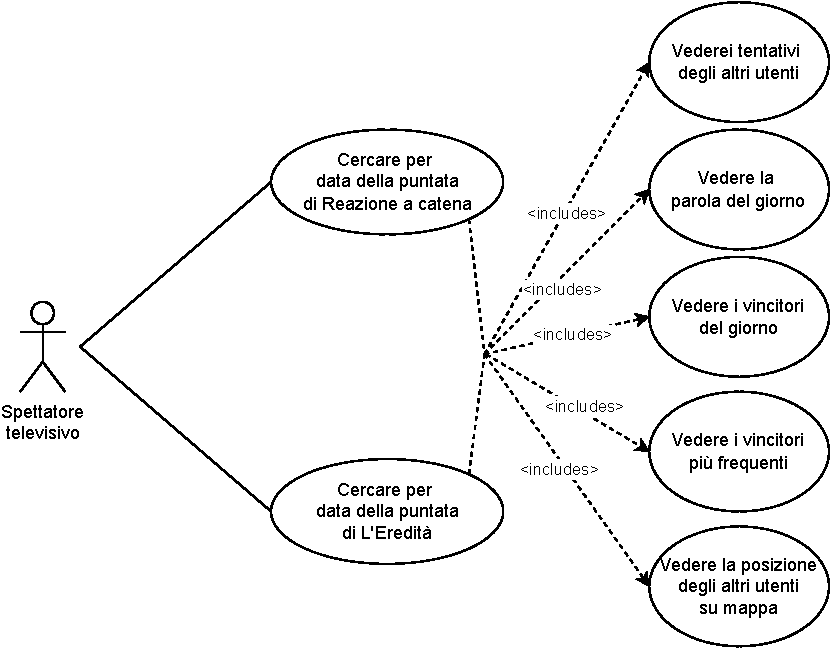
\includegraphics[scale=0.7]{./img/usecase/tvgames.pdf}
    \caption{Casi d'uso per l'epica: Giochi televisivi}
\end{figure}

\begin{figure}[H]
    \centering
    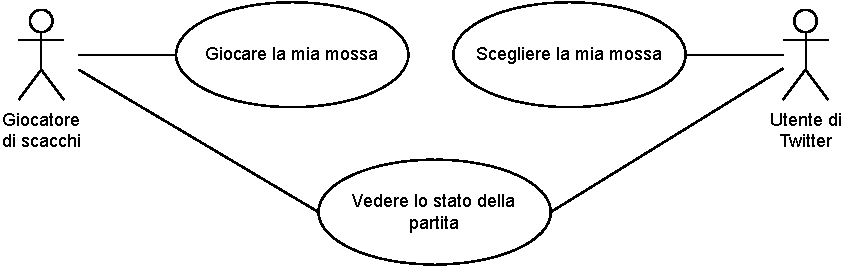
\includegraphics[scale=0.7]{./img/usecase/chess.pdf}
    \caption{Casi d'uso per l'epica: Scacchi}
\end{figure}

\begin{figure}[H]
    \centering
    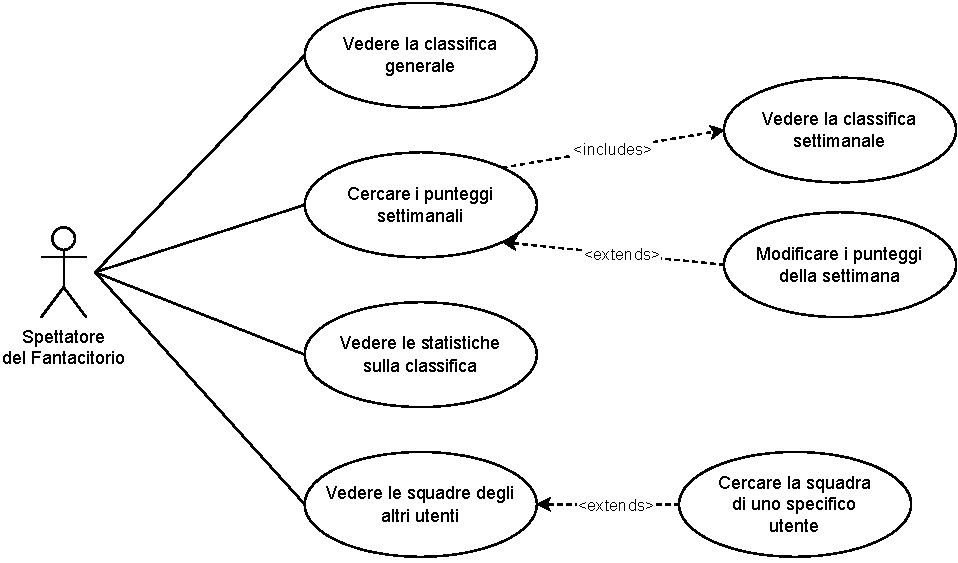
\includegraphics[scale=0.7]{./img/usecase/fantacitorio.pdf}
    \caption{Casi d'uso per l'epica: Fantacitorio}
\end{figure}


\subsection{Diagramma delle classi}
Di seguito sono descritti, sottoforma di schede CRC, gli oggetti e le funzioni suddivisi per epica del backlog.\\
Per molte funzionalità del prodotto, si è ritenuto più adatto seguire un approccio funzionale (divisi in moduli) invece di utilizzare un approccio a oggetti.\\
Nonostante ciò, si è preferito descrivere la progettazione come schede CRC, anche se le entità non sono propriamente classi,
in quanto per ciascun modulo è possibile individuare le responsabilità e le dipendenze.

\subsubsection*{Raccolta e analisi di tweet}
%%% Raccolta
\crc{fetch/keyword}{%
    \item Raccolta di tweet per parola chiave
}{%
}

\crc{fetch/user}{%
    \item Raccolta di tweet per nome utente
}{%
}

\crc{fetch/multiple\_tweets}{%
    \item Raccolta di un determinato numero (potenzialmente alto) di tweet
}{%
    \item \texttt{fetch/keyword}
    \item \texttt{fetch/user}
}

\crc{fetch/stream}{%
    \item Apertura di uno stream per la raccolta di tweet in tempo reale
    \item Lettura dallo stream
    \item Chiusura dello stream
}{%
}

%%% Analisi
\crc{analysis/language}{%
    \item Rilevazione della lingua di un testo
}{%
}

\crc{analysis/sentiment}{%
    \item Rilevazione del sentimento di un testo
}{%
    \item \texttt{analysis/language}
}

\crc{analysis/stopwords}{%
    \item Rimozione di stop words da un testo
}{%
    \item \texttt{analysis/language}
}


\subsubsection*{Scacchi}

\crc{tweet/twitter\_oauth}{%
    \item Autenticazione a Twitter
}{%
}

\crc{tweet/send}{%
    \item Pubblicazione di un tweet
}{%
    \item \texttt{tweet/twitter\_oauth}
}

\crc{ChessOpponent}{%
    \item Pubblicazione dell'immagine con lo stato della scacchiera
    \item Selezione della mossa successiva a maggioranza
}{%
    \item \texttt{tweet/send}
}

\crc{ChessGame}{%
    \item Tracciamento dello stato della partita
    \item Rilevamento conclusione partita
}{%
}

\subsubsection*{Reazione a catena e L'Eredità}
\crc{games/winningWord}{%
    \item Estrazione della parola vincente
}{%
    \item \texttt{fetch/keyword}
}
\crc{games/userAttempts}{%
    \item Raccolta dei tentativi degli utenti
}{%
    \item \texttt{fetch/keyword}
}

\subsubsection*{Fantacitorio}
\crc{games/fantacitorio}{%
    \item Raccolta dei punteggi settimanali
    \item Calcolo della classifica generale
    \item Raccolta delle squadre degli utenti
    \item Calcolo di statistiche sulla classifica
}{%
    \item \texttt{fetch/keyword}
    \item \texttt{fetch/user}
}


%%%

\newpage
\section{Descrizione degli sprint} \label{sprint_description}
Sono stati svolti quattro sprint della durata di 14 giorni ciascuno.\\
La stima dei punti delle user stories è stata effettuata con una scala da 0 a 10, valutando separatamente il frontend dal backend. 
Il punteggio complessivo è quindi ottenuto dalla somma di quest'ultimi.

\subsection{Sprint 1}
\subsubsection{Sprint goal}
Lo sprint è stato principalmente dedicato a studiare le API di Twitter e produrre le prime funzionalità per la visualizzazione e l'analisi dei tweet.\\
In particolare le feature pianificate per lo sprint sono state:
\begin{itemize}
    \item Ricerca di tweet per username
    \item Ricerca di tweet per hashtag
    \item Analisi dei tweet tramite componenti grafiche:
    \begin{itemize}
        \item Grafico a torta per l'analisi del sentimento
        \item Grafico a barre per la frequenza dei tweet
        \item Word cloud con le parole più usate
    \end{itemize}
\end{itemize}


\subsubsection{Backlog}
\userstory%
{Come utente interessato ai tweet,\\voglio poter cercare dei tweet per hashtag\\per leggerli.}%
{8\\(3 frontend + 5 backend)}%
{L'utente, cercando un hashtag in un apposito textbox, è in grado di leggere tutti i tweet correlati visualizzando:
nome account Twitter, username, immagine profilo, contenuto tweet (testo + foto e video), data e ora, luogo (se applicabile), numero like, numero commenti, numero retweet.}%
{Richiamare l'API implementata, verificare che il formato sia corretto e che il contenuti dei tweet contenga l'hashtag ricercato.}
{Raccolta e analisi di tweet}

\userstory%
{Come utente interessato ai tweet,\\voglio poter cercare dei tweet per nome utente\\per leggerli.}%
{8\\(3 frontend + 5 backend)}%
{L'utente, cercando un nome utente in un apposito textbox, è in grado di leggere tutti i tweet correlati visualizzando:
nome account Twitter, username, immagine profilo, contenuto tweet (testo + foto e video), data e ora, luogo (se applicabile), numero like, numero commenti, numero retweet.}%
{Richiamare l'API implementata, verificare che il formato sia corretto e che l'autore dei tweet sia quello ricercato.}
{Raccolta e analisi di tweet}

\userstory%
{Come analista,\\voglio poter analizzare il sentimento\\per stabilire se un tweet è positivo o meno.}%
{9\\(2 frontend + 7 backend)}%
{L'utente, dato un tweet, vede se è positivo, negativo o neutro tramite immagine o testo.}%
{Analizzare frasi di cui è noto il sentimento.}
{Raccolta e analisi di tweet}

\userstory%
{Come analista,\\voglio vedere un grafico a barre\\per vedere il numero di tweet nell'unità di tempo.}%
{2\\(2 frontend)}%
{L'utente apre una pagina web contenente il grafico a barre con il numero di tweet nell'unità di tempo.}%
{Manualmente verificare che il grafico sia corretto.}
{Raccolta e analisi di tweet}

\userstory%
{Come analista,\\voglio vedere un grafico a torta\\per vedere il rapporto di sentiment positivi, negativi e neutri.}%
{2\\(2 frontend)}%
{L'utente apre una pagina web contenente il grafico a torta con sentiment positivi, negativi e neutri.}%
{Manualmente verificare che il grafico sia corretto.}
{Raccolta e analisi di tweet}

\userstory%
{Come analista,\\voglio vedere una term cloud\\per vedere le parole più utilizzate nei tweet.}%
{4\\(2 frontend + 2 backend)}%
{L'utente apre una pagina web contenente una term cloud con le parole più utilizzate.}%
{Manualmente verificare che il grafico sia corretto.}
{Raccolta e analisi di tweet}

\newpage
\subsubsection{Esito sprint}
Lo sprint è terminato con la conclusione di tutte le user stories pianificate.\\
Il lavoro è risultato omogeneo, con un piccolo scostamento rispetto all'andamento ideale 
che però non è stato causa di imprevisti o ritardi.\\
\begin{figure}[H]
    \centering
    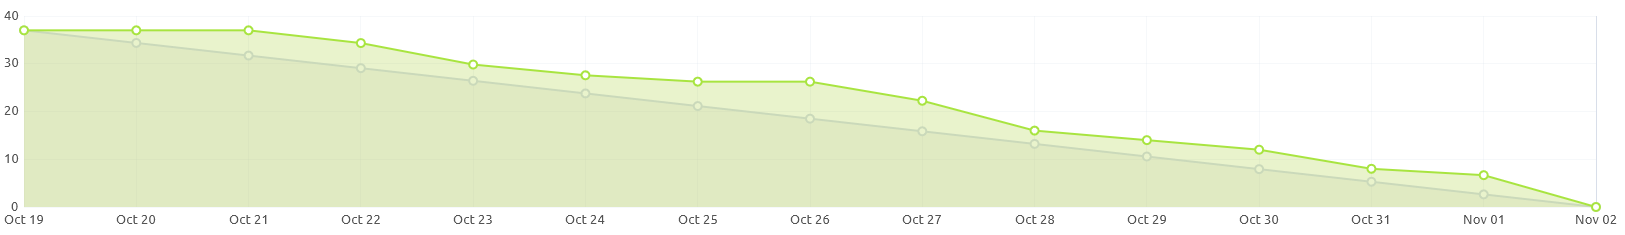
\includegraphics[width=15cm]{./img/sprint1/burndown.png}
    \caption{Burndown sprint 1}
\end{figure}
Anche le ore di lavoro (con il tempo stimato in quanto allo sprint 1 non è stato effettuato il monitoraggio) sono risultate in linea con il monte ore previsto.\\
\begin{figure}[H]
    \centering
    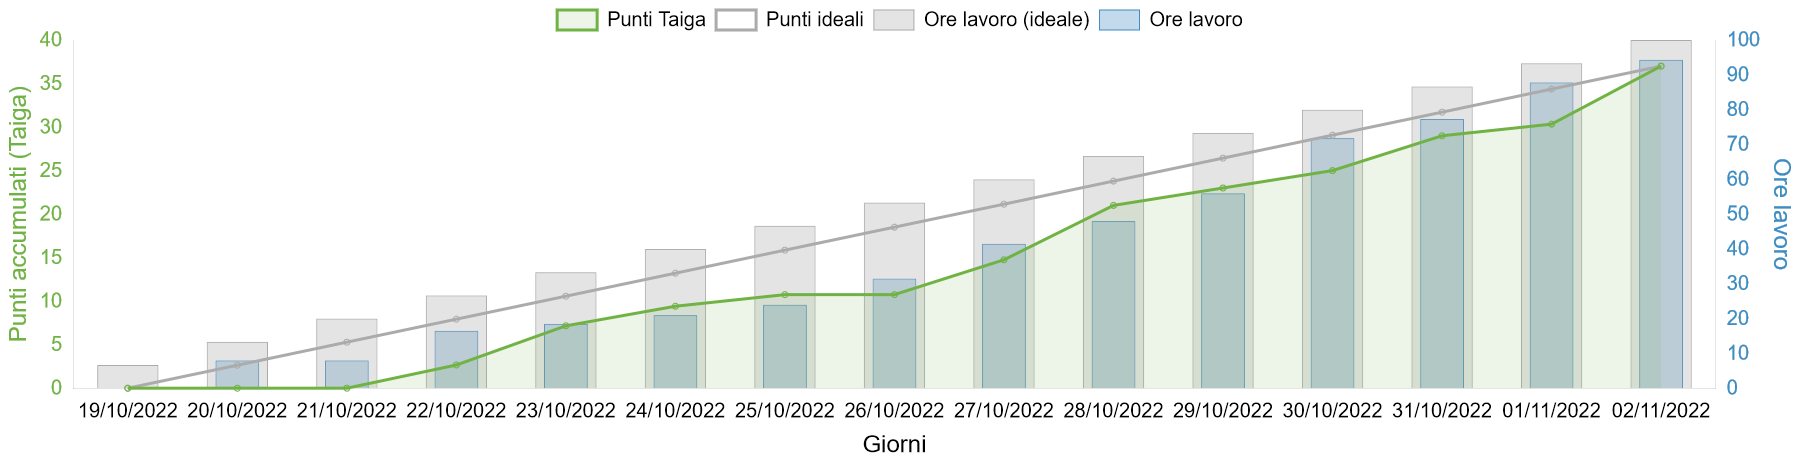
\includegraphics[width=15cm]{./img/sprint1/worktime.png}
    \caption{Progresso dei punti (asse a sinistra) e ore di lavoro (asse a destra)}
\end{figure}


\subsubsection{Sprint review}
Alla sprint review è stato chiesto dal cliente l'implementazione delle seguenti feature:
\begin{itemize}
    \item Ricerca di tweet per intervallo temporale
    \item Possibilità di selezionare il numero di tweet da estrare con una singola richiesta
\end{itemize}


\subsubsection{Retrospettiva}
\subsubsection*{Pre-retrospettiva}
Alla pre-retrospettiva effettuata a metà sprint, sono emerse le seguenti problematiche:
\begin{itemize}
    \item Tempo dedicato al lavoro non sufficiente
    \item Mancanza di comunicazione nel team
    \item Task e user stories hanno descrizioni poco dettagliate e facilmente fraintendibili
\end{itemize}
\begin{figure}[H]
    \centering
    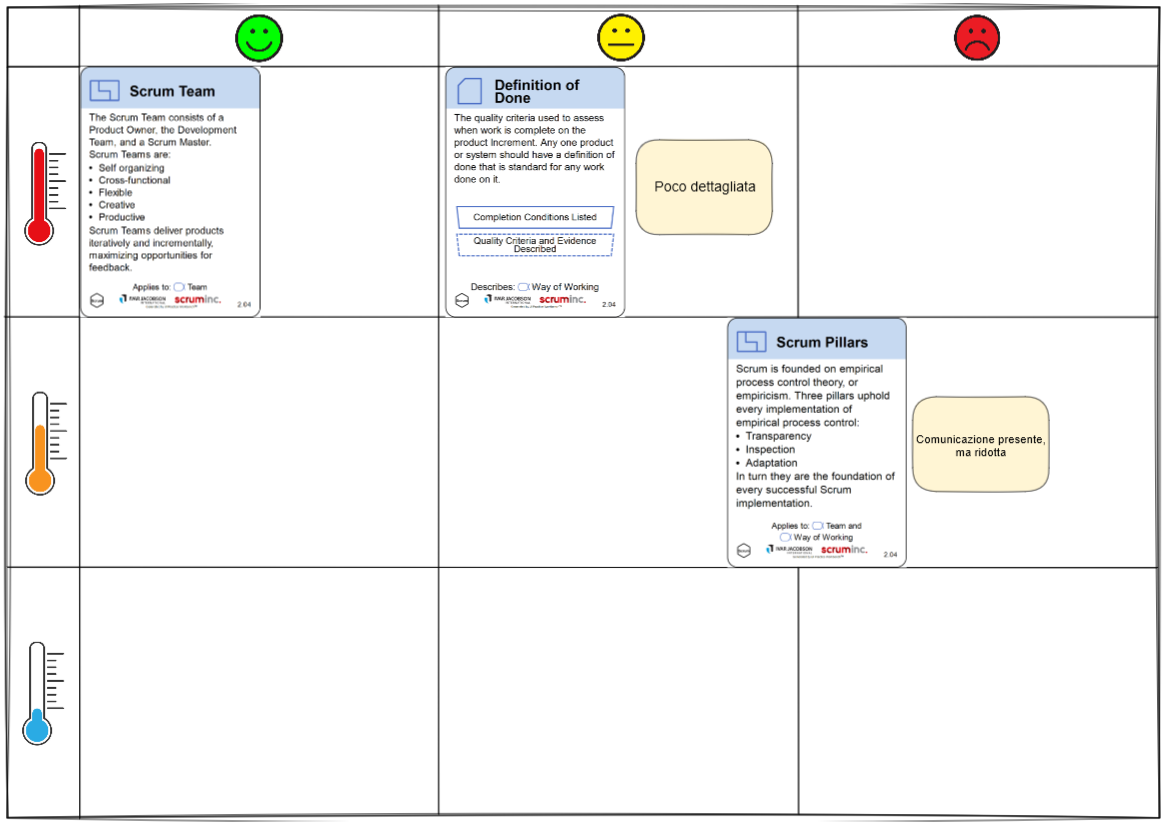
\includegraphics[width=15cm]{./img/sprint1/preretrospettiva.png}
    \caption{Pre-retrospettiva del 27/10/2022}
\end{figure}

\subsubsection*{Retrospettiva}
Alla retrospettiva di fine sprint, gli aspetti positivi evidenziati dal team sono:
\begin{itemize}
    \item Il deliverable presentato alla sprint review è risultato adeguato e funzionante
    \item Il team e i ruoli di ciascuno sono ben definiti
\end{itemize}
Sono invece stati portati all'attenzione del team i seguenti problemi:
\begin{itemize}
    \item Non è stato effettuato un monitoraggio delle ore di lavoro (che è stato quindi stimato sulla base sui daily scrum virtuali)
    \item I problemi evidenziali alla pre-retrospettiva non sono ancora stati risolti 
\end{itemize}
\begin{figure}[H]
    \centering
    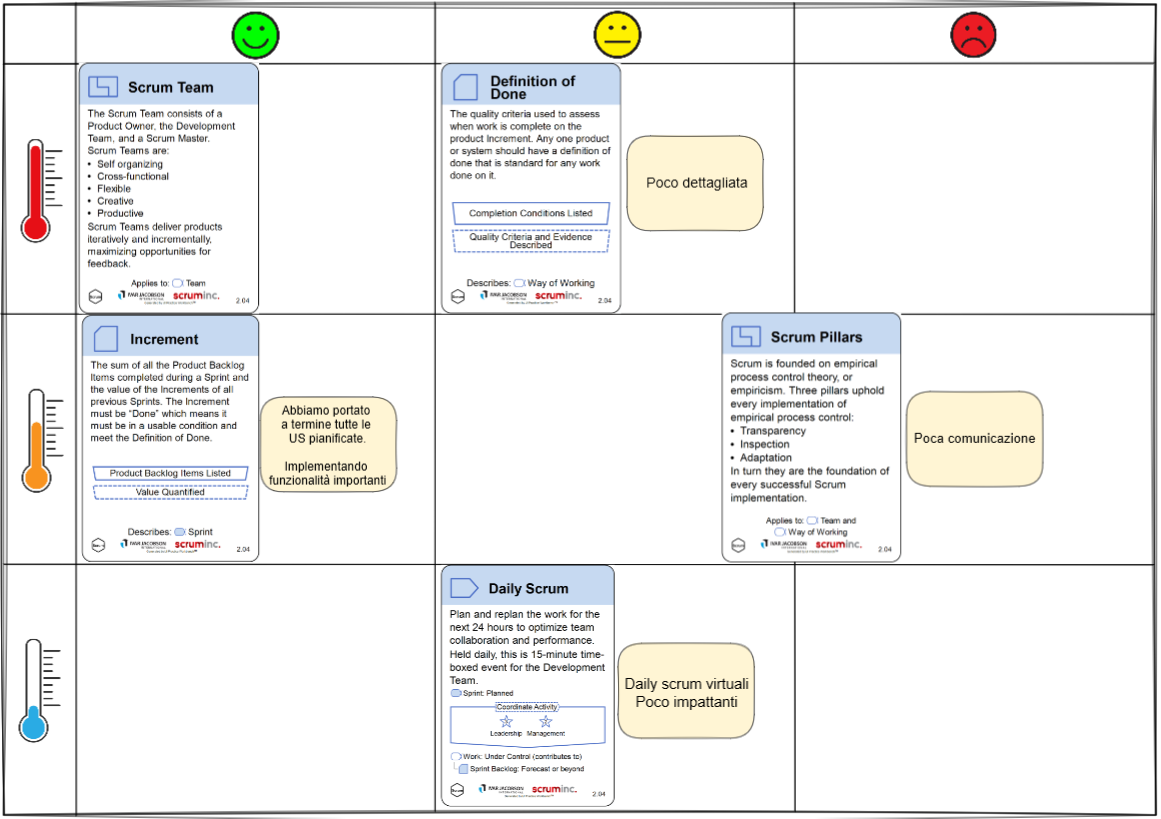
\includegraphics[width=15cm]{./img/sprint1/retrospettiva.png}
    \caption{Retrospettiva del 01/11/2022}
\end{figure}
\newpage

\subsection{Sprint 2}
\subsubsection{Sprint goal}
L'obiettivo dello sprint è stato quello di concludere l'epica riguardante la visualizzazione e l'analisi dei tweet.\\
Nello specifico, sono state implementate le seguenti funzionalità:
\begin{itemize}
    \item Ricerca di tweet per intervallo temporale (richiesto dal cliente allo sprint review precedente)
    \item Ricerca di un determinato numero di tweet con una singola ricerca (richiesto dal cliente allo sprint review precedente)
    \item Ricerca di tweet per parola chiave
    \item Mappa per visualizzare la posizione dei tweet con geolocalizzazione
    \item Raccolta di tweet in tempo reale
\end{itemize}


\subsubsection{Backlog}
\userstory%
{Come utente interessato a vedere tweet,\\voglio scegliere un numero di tweet da poter caricare in una volta\\per poterli analizzare in modo aggregato.}%
{5\\(3 frontend + 2 backend)}%
{Possibilità di ricercare un largo numero di tweet scrivendone la quantità in un textbox.\\
Tale quantità serve per la ricerca iniziale e anche per mostrare pagine successive. 
È possibile inoltre ricercare un numero di tweet inizialmente per poi cambiare quantità e cercare una pagina successiva 
(esempio: ricerca di 150 tweet iniziali, poi viene modificata la quantità (dallo stesso textbox) in 20 e si preme su “Pagina successiva”. Il numero di tweet così mostrato diventa 170).}%
{Verificare che il numero di tweet raccolto corrisponda con quello richiesto.}
{Raccolta e analisi di tweet}

\userstory%
{Come utente interessato a vedere tweet,\\voglio scegliere un intervallo di tempo in cui raccogliere tweet\\per analizzarne le tendenze storiche.}%
{5\\(3 frontend + 2 backend)}%
{Possibilità di ricercare dei tweet dato un intervallo temporale. Non deve essere possibile cercare tweet nel futuro.\\
Non deve essere possibile cliccare su “Prossima pagina” quando non ci sono più tweet da visualizzare.}%
{Verificare che i tweet raccolti siano compresi nell'intervallo temporale.}
{Raccolta e analisi di tweet}

\userstory%
{Come utente interessato a vedere tweet,\\voglio poter cercare dei tweet per parola chiave\\per vedere cosa ne pensa la gente a riguardo.}%
{4\\(2 frontend + 2 backend)}%
{Possibilità di cercare tweet per parola o frase chiave. I grafici già presenti devono funzionare anche con questa ricerca.}%
{Richiamare l'API implementata, verificare che il formato sia corretto e che il contenuti dei tweet contenga la parola chiave ricercata.}
{Raccolta e analisi di tweet}

\userstory%
{Come utente interessato ai tweet,\\voglio poter visualizzare su una mappa la posizione dei tweet cercati\\per avere un'idea della località dalla quale sono stati pubblicati.}%
{7\\(3 frontend + 4 backend)}%
{Possibilità di visualizzare una mappa con le posizioni dei tweet ricercati.\\
Se sono presenti più tweet nella stessa zona è possibile aggregarli (in base alla distanza) e mostrare un unico valore, 
ovvero il numero di tweet in tale zona. La mappa deve essere sempre visibile anche durante lo scorrimento della pagina (come i grafici).}%
{Manualmente verificare che la mappa contenga i marker quando sono presenti tweet con geolocalizzazione.}
{Raccolta e analisi di tweet}

\userstory%
{Come utente,\\voglio vedere la posizione di tutti i tweet di una data persona\\per conoscere i suoi spostamenti.}%
{5\\(5 frontend + 0 backend)}%
{Possibilità di inserire il nome utente di una persona e visualizzare su una mappa le posizioni dei suoi tweet e i suoi spostamenti.\\
Per gli spostamenti si mostrano sulla mappa delle frecce basandosi sulla posizione e sulla data del tweet.}%
{Manualmente verificare che la mappa contenga i marker quando sono presenti tweet con geolocalizzazione.}
{Raccolta e analisi di tweet}

\userstory%
{Come lettore di tweet,\\voglio poter vedere i tweet che ricerco in tempo reale\\per sapere cosa la gente posta.}%
{10\\(3 frontend + 7 backend)}%
{Poter scrivere una ricerca e, al click di un pulsante “Live”, vedere tutti i tweet pubblicati in tempo reale a partire da quel momento.}%
{Verificare che il socket implementato restituisca i tweet ricercati, quando disponibili.}
{Raccolta e analisi di tweet}

\newpage
\subsubsection{Esito sprint}
Lo sprint è terminato con la conclusione di tutte le user stories pianificate.\\
Il lavoro si è svolto in linea con l'andamento ideale dei punti. 
Si è osservato una leggera sovrastima delle user stories che ha portato alla conclusione anticipata (di un giorno) dello sprint.\\
\begin{figure}[H]
    \centering
    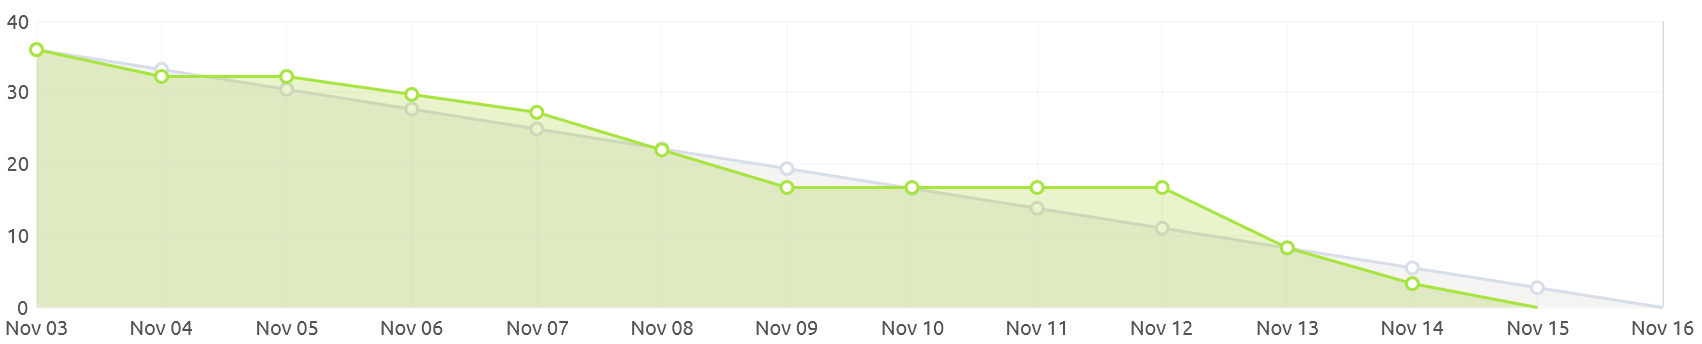
\includegraphics[width=15cm]{./img/sprint2/burndown.png}
    \caption{Burndown sprint 2}
\end{figure}
Le ore di lavoro rispettano il monte ore e sono state distribute principalmente in due periodi di maggiore produttività.
\begin{figure}[H]
    \centering
    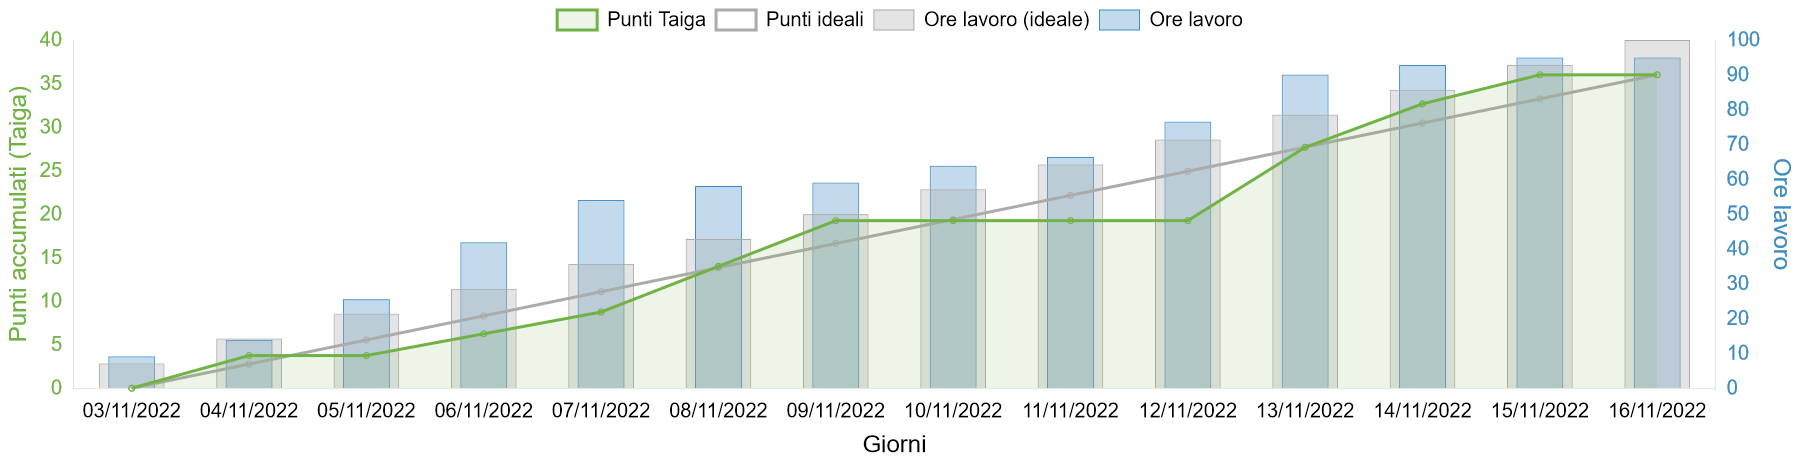
\includegraphics[width=15cm]{./img/sprint2/worktime.png}
    \caption{Progresso dei punti (asse a sinistra) e ore di lavoro (asse a destra)}
\end{figure}


\subsubsection{Sprint review}
Alla sprint review non sono emerse nuove richieste da parte del cliente.


\newpage
\subsubsection{Retrospettiva} \label{sprint1_retrospettiva}
\subsubsection*{Pre-retrospettiva}
Alla pre-retrospettiva effettuata a metà sprint, sono emerse le seguenti problematiche:
\begin{itemize}
    \item Mancanza di test adeguati per il frontend
    \item Le user stories sono state sovrastimate
\end{itemize}
\begin{figure}[H]
    \centering
    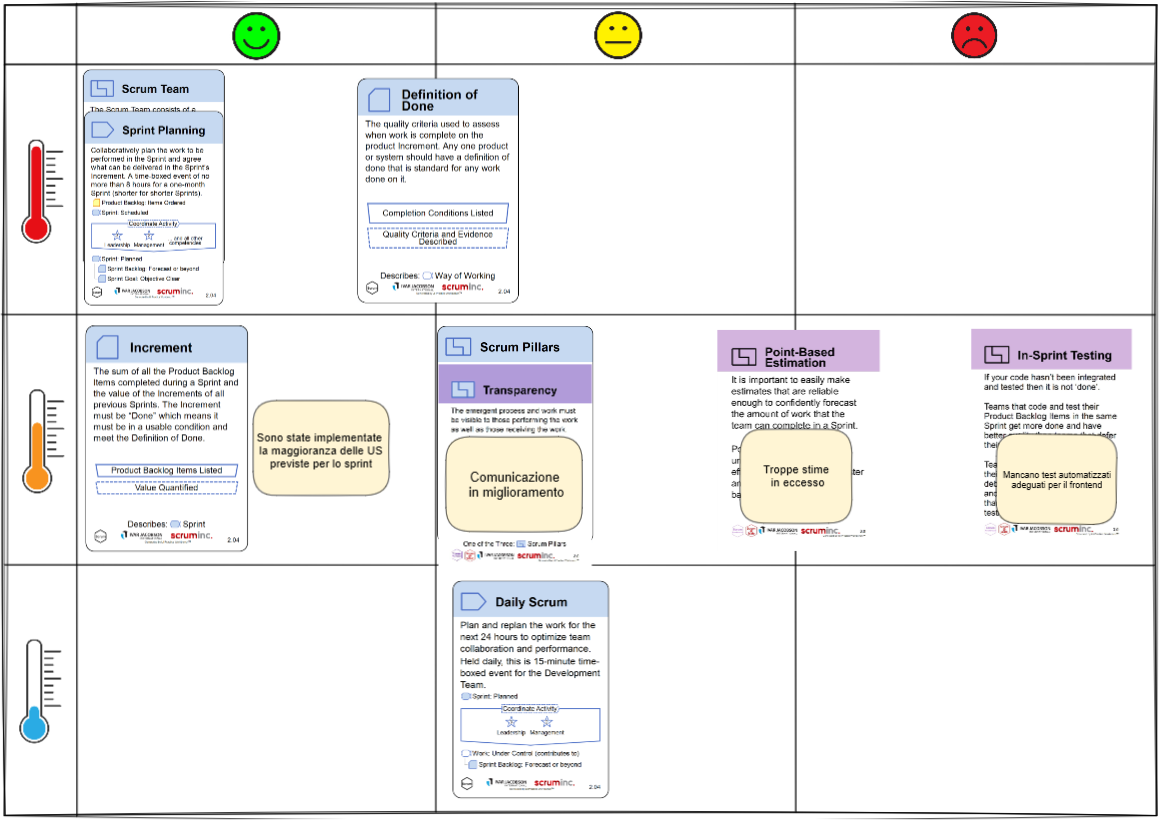
\includegraphics[width=15cm]{./img/sprint2/preretrospettiva.png}
    \caption{Pre-retrospettiva del 10/11/2022}
\end{figure}

\subsection*{Retrospettiva}
Alla retrospettiva di fine sprint sono state confermate le problematiche della pre-retrospettiva.
\newpage

\subsection{Sprint 3}
\subsubsection{Sprint goal}

\subsubsection{Backlog}
\userstory%
{Come spettatore de \#leredita\\voglio raccogliere i tweet di chi prova a indovinare la ghigliottina,\\per visualizzare, in ordine temporale, tutti coloro che provano ad indovinare.}%
{5\\(2 frontend + 3 backend)}%
{Possibilità di visualizzare una pagina con tutti i tweet di tutte le persone che usano l'\#leredita e provano ad indovinare la ghigliottina.}%
{Cercando per data, verificare che vengano visualizzati i tentativi del giorno}

\userstory%
{Come spettatore de \#leredita\\voglio visualizzare, su una mappa, la posizione di tutti coloro che provano ad indovinare\\per conoscere la posizione di giocatori.}%
{4\\(4 frontend)}%
{Possibilità di visualizzare una pagina con tutte le posizioni su una mappa di tweet di tutte le persone che usano l'\#leredita e provano ad indovinare la ghigliottina.}%
{Manualmente verificare che nella mappa siano presenti i marker dei tweet con la geolocalizzazione}

\userstory%
{Come spettatore de \#leredita\\voglio visualizzare tutti coloro che indovinano la ghigliottina\\per sapere chi ha indovinato.}%
{7\\(4 frontend + 3 backend)}%
{Possibilità di visualizzare la parola del giorno assieme a tutti i vincitori che hanno indovinato.}%
{Cercando per data, verificare che venga trovata la parola del giorno}

\userstory%
{Come spettatore di \#reazioneacatena\\voglio raccogliere i tweet di chi prova a indovinare l'ultima parola,\\per visualizzare, in ordine temporale, tutti coloro che provano ad indovinare.}%
{2\\(2 backend)}%
{Possibilità di visualizzare una pagina con tutti i tweet di tutte le persone che usano l'\#reazioneacatena e provano ad indovinare la parola finale.}%
{Cercando per data, verificare che vengano visualizzati i tentativi del giorno}

\userstory%
{Come spettatore di \#reazioneacatena\\voglio visualizzare, su una mappa, la posizione di tutti coloro che provano ad indovinare\\per conoscere la posizione di giocatori.}%
{0}%
{Possibilità di visualizzare una pagina con tutte le posizioni su una mappa di tweet di tutte le persone che usano l'\#reazioneacatena e provano ad indovinare la parola finale.}%
{Manualmente verificare che nella mappa siano presenti i marker dei tweet con la geolocalizzazione}

\userstory%
{Come spettatore de \#reazioneacatena\\voglio visualizzare tutti coloro che indovinano l'ultima parola\\per sapere chi ha indovinato.}%
{2\\(0 frontend + 2 backend)}%
{Possibilità di visualizzare la parola del giorno assieme a tutti i vincitori che hanno indovinato.}%
{Cercando per data, verificare che venga trovata la parola del giorno}

\userstory%
{Come giocatore di scacchi\\Voglio poter muovere una pedina\\Per fare la mia mossa}%
{12\\(6 frontend + 6 backend)}%
{Possibilità di fare una mossa a scacchi e visualizzarla}%
{Provare a effettuare mosse valide e invalide}

\subsubsection{Burndown}
\begin{figure}[H]
    \centering
    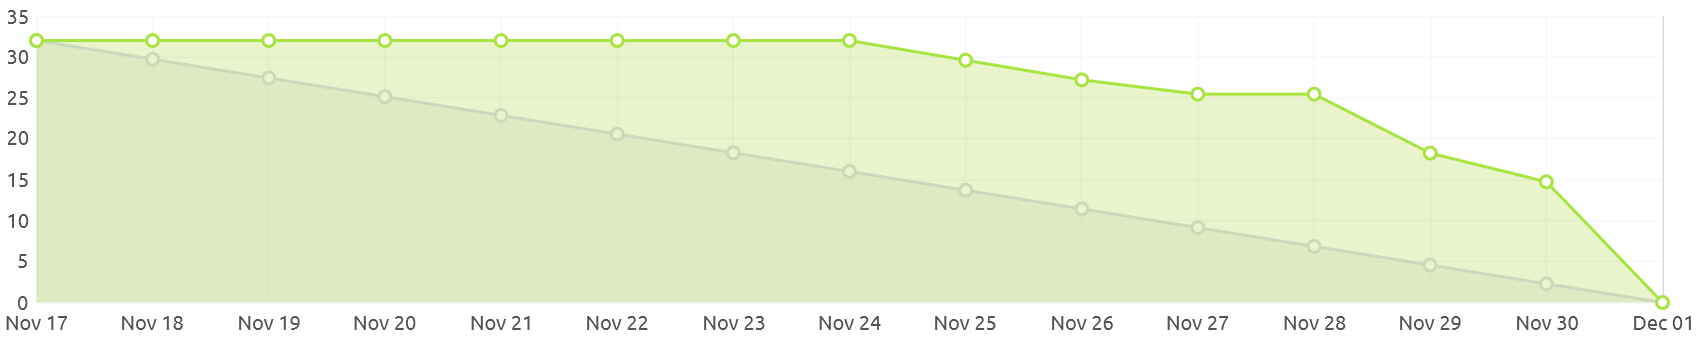
\includegraphics[width=15cm]{./img/sprint3/burndown.png}
    \caption{Burndown}
\end{figure}
\begin{figure}[H]
    \centering
    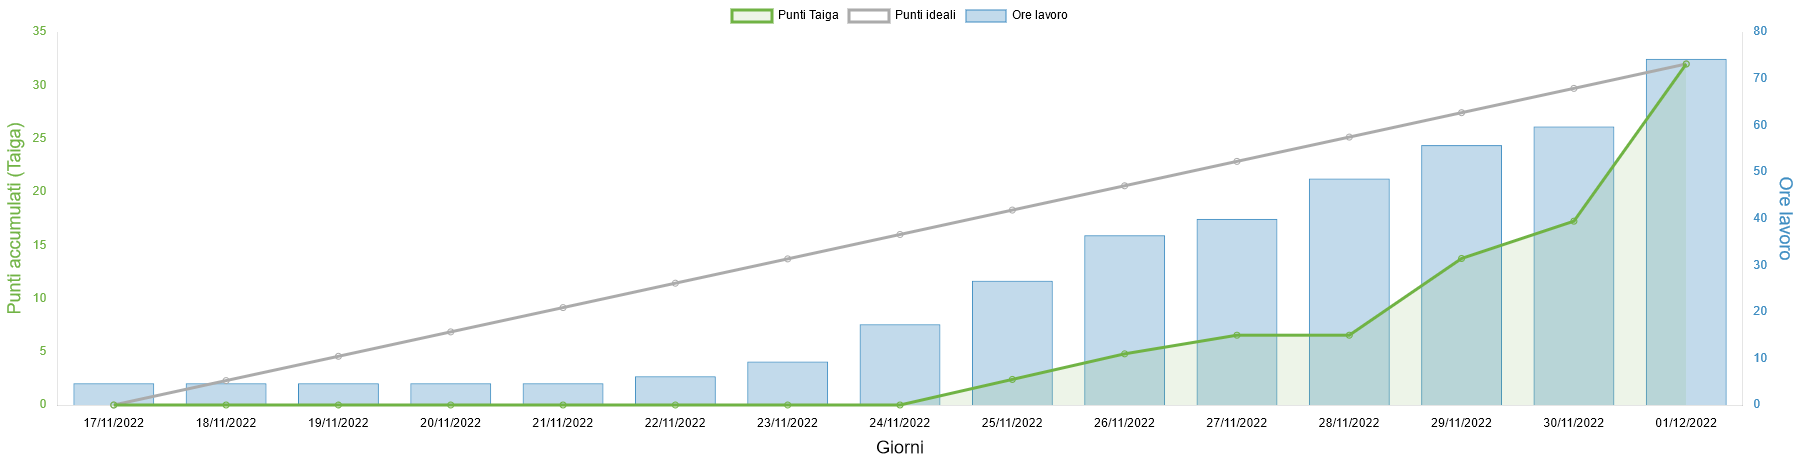
\includegraphics[width=15cm]{./img/sprint3/worktime.png}
    \caption{Progresso dei punti (asse a sinistra) e ore di lavoro (asse a destra)}
\end{figure}

\subsubsection{Retrospettiva}
\begin{figure}[H]
    \centering
    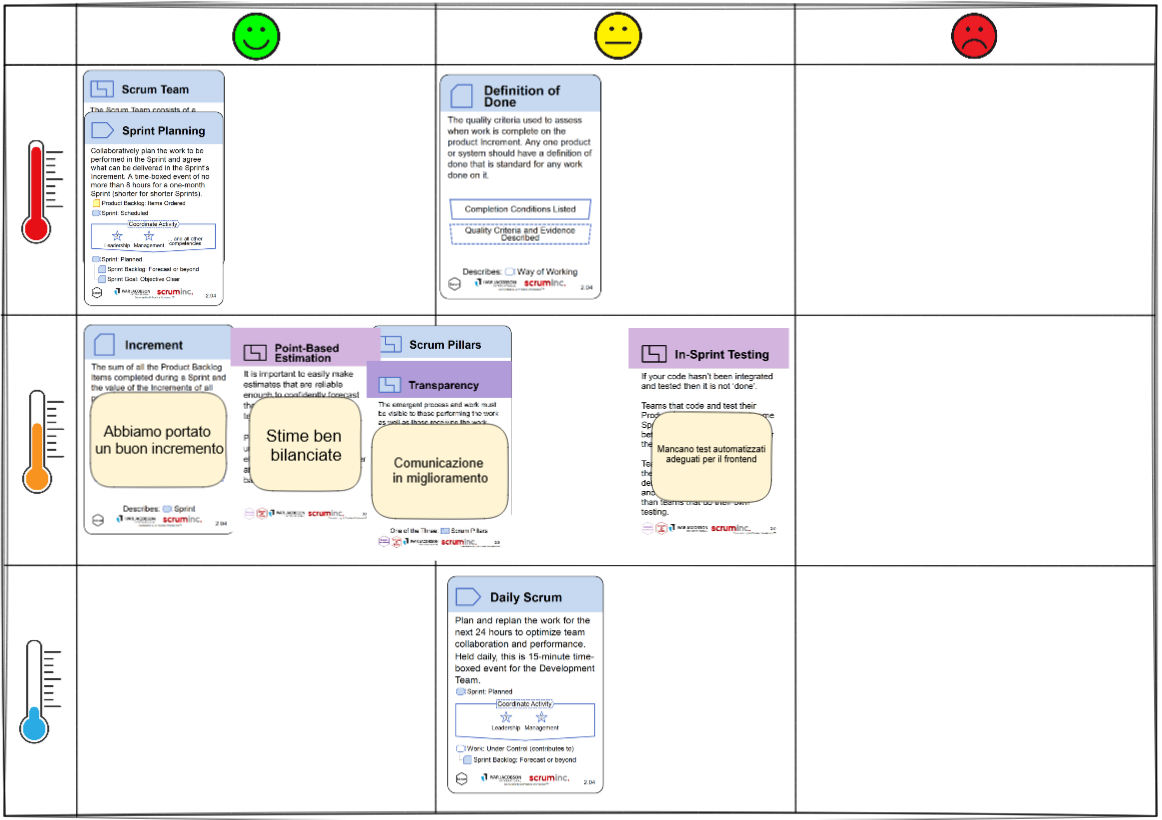
\includegraphics[width=15cm]{./img/sprint3/retrospettiva.png}
    \caption{Pre-retrospettiva del 02/12/2022}
\end{figure}

\newpage

\subsection{Sprint 4}
\subsubsection{Sprint goal}
L'obiettivo dello sprint finale è stato quello di implementare il Fantacitorio (richiesto allo sprint precedente), concludere lo scacchi e 
integrare le richieste del cliente emerse dalla sprint review precedente nel prodotto finale.\\
In particolare sono state previste le seguenti funzionalità:
\begin{itemize}
    \item Per il Fantacitorio:
    \begin{itemize}
        \item Visualizzazione e modifica della classifica settimanale
        \item Visualizzazione della classifica generale
        \item Visualizzazione delle squadre degli altri giocatori
        \item Ricerca della squadra di uno specifico utente
        \item Statistiche sulla classifica
    \end{itemize}
    \item Per lo scacchi:
    \begin{itemize}
        \item Pubblicazione della scacchiera come tweet
        \item Raccolta e selezione della mossa dell'avversario a maggioranza
    \end{itemize}
    \item Per i giochi televisivi:
    \begin{itemize}
        \item Visualizzazione dei più vincenti in un periodo di tempo
    \end{itemize}
\end{itemize}


\subsubsection{Backlog}
\userstory%
{Come interessato al Fantacitorio,\\voglio vedere e poter aggiornare una sintesi settimanale dei punteggi dei politici\\per vedere chi sta vincendo.}%
{11\\(4 frontend + 7 backend)}%
{Avere una lista di tutti i politici con i loro relativi punteggi, visualizzarne una sintesi e poter modificarla.}%
{Verificare il corretto parsing dei tweet contentente i punteggi.}

\userstory%
{Come interessato al Fantacitorio,\\voglio vedere una classifica cumulativa di punteggi di ogni politico\\per capire chi sta vincendo.}%
{5\\(2 frontend + 3 backend)}%
{Visualizzare una classifica cumulativa con i punti di ogni politico in ordine decrescente.}%
{Verificare che la classifica sia coerente con i punteggi settimanali.}

\userstory%
{Come interessato al Fantacitorio,\\voglio sfogliare le immagini delle squadre degli altri partecipanti\\per vedere contro chi competo.}%
{7\\(3 frontend + 4 backend)}%
{Visualizzare, in una pagina, tutte le foto delle squadre partecipanti al Fantacitorio.}%
{Verificare manualmente che l'algoritmo sia in grado di riconoscere correttamente le immagini contenente una squadra.}

\userstory%
{Come interessato al Fantacitorio,\\voglio poter cercare un utente e vedere se partecipa o meno e mostrare la sua squadra\\per cercare chi gioca.}%
{5\\(2 frontend + 3 backend)}%
{Possibilità di cercare un utente per username e controllare se possiede una squadra, in caso affermativo mostrarla.}%
{Verificare che cercando un utente che partecipa al Fantacitorio, la sua squadra sia visibile.}

\userstory%
{Come giocatore di scacchi,\\voglio che la scacchiera venga pubblicata\\in modo tale che gli utenti vedano la mossa scelta.}%
{3\\(3 backend)}%
{Pubblicare un tweet con la foto della scacchiera allo stato attuale.}%
{Verificare manualmente che il tweet sia stato pubblicato.}

\userstory%
{Come giocatore di scacchi,\\voglio che gli utenti di Twitter scelgano, a maggioranza, la mossa dell'avversario\\per avanzare nella partita.}%
{4\\(1 frontend + 3 backend)}%
{Scelta di una mossa in base alla maggioranza dei voti presenti nei commenti del post pubblicato.}%
{Verificare che la mossa scelta sia quella proposta dal maggior numero di utenti.}

\userstory%
{Come spettatore de \#leredita,\\voglio visualizzare colui/colei che ha indovinato più volte nel corso delle puntate,\\per sapere chi è più bravo/a.}%
{5\\(2 frontend + 3 backend)}%
{Possibilità di visualizzare, giorno per giorno, una classifica con le persone con più parole indovinate.}%
{Verificare che gli utenti visualizzati abbiano effettivamente vinto il numero di volte indicato.}

\userstory%
{Come spettatore de \#reazioneacatena,\\voglio visualizzare colui/colei che ha indovinato più volte nel corso delle puntate,\\per sapere chi è più bravo/a.}%
{1\\(1 backend)}%
{Possibilità di visualizzare, giorno per giorno, una classifica con le persone con più parole indovinate.}%
{Verificare che gli utenti visualizzati abbiano effettivamente vinto il numero di volte indicato.}

\userstory%
{Come interessato al Fantacitorio,\\voglio visualizzare delle statistiche interessanti nella classifica\\per vedere chi sta andando bene e chi no.}%
{3\\(1 frontend + 2 backend)}%
{Mostrare statistiche interessanti nella pagina della classifica, come ad esempio “best climber”, “best average” e “best single score”.}%
{Verificare che le statistiche siano in linea con la classifica.}


\subsubsection{Esito sprint}
Lo sprint è terminato con la conclusione di tutte le user stories pianificate.\\
\begin{figure}[H]
    \centering
    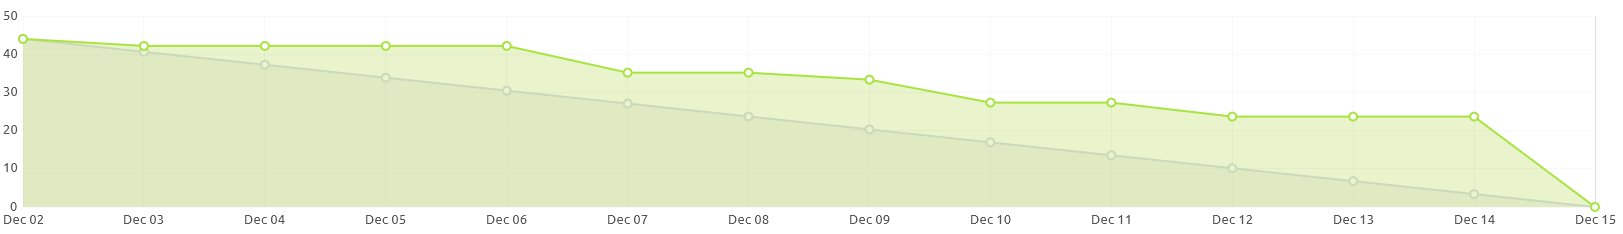
\includegraphics[width=15cm]{./img/sprint4/burndown.png}
    \caption{Burndown sprint 4}
\end{figure}
La distribuzione delle ore di lavoro è risultata disomogenea, con un'importante concentrazione all'ultimo giorno dello sprint.
\begin{figure}[H]
    \centering
    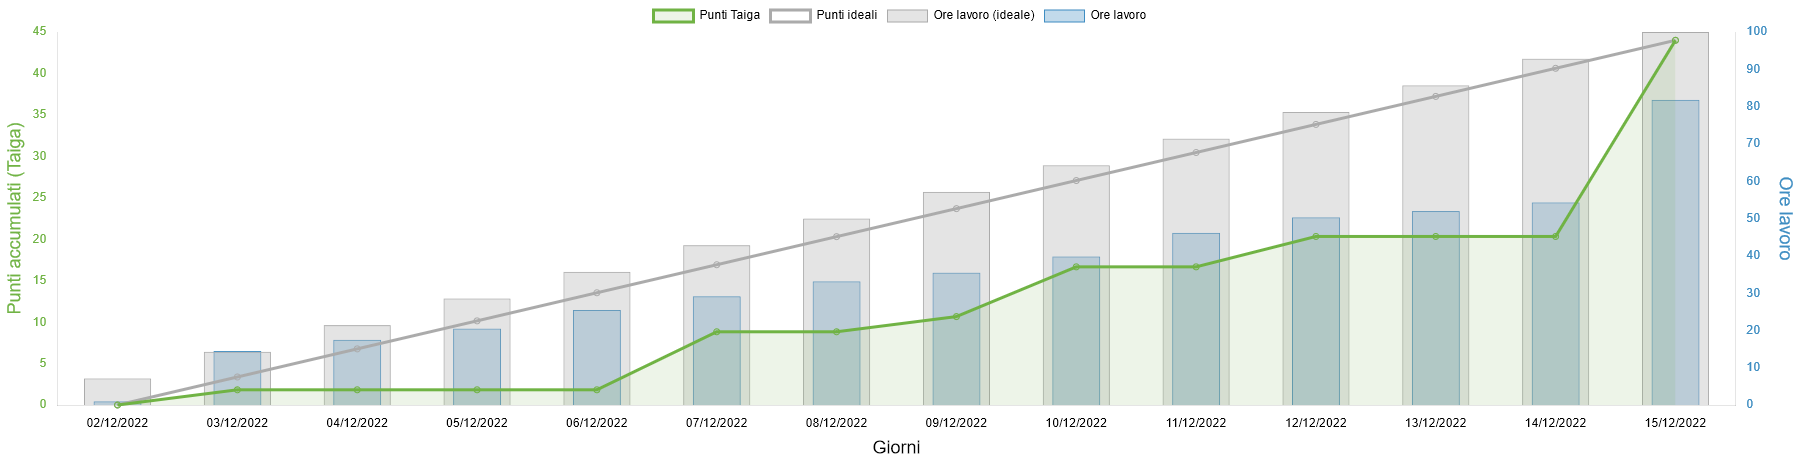
\includegraphics[width=15cm]{./img/sprint4/worktime.png}
    \caption{Progresso dei punti (asse a sinistra) e ore di lavoro (asse a destra)}
\end{figure}


\newpage
\subsubsection{Retrospettiva}
Alla retrospettiva il team ha evidenziato i seguenti aspetti positivi:
\begin{itemize}
    \item Una buona reazione alle modifiche del backlog
    \item Un incremento significativo nei test (del frontend)
\end{itemize}
È stato invece evidenziato come aspetto negativo un mal bilanciamento del lavoro, concentrato tutto alla fine dello sprint.
\begin{figure}[H]
    \centering
    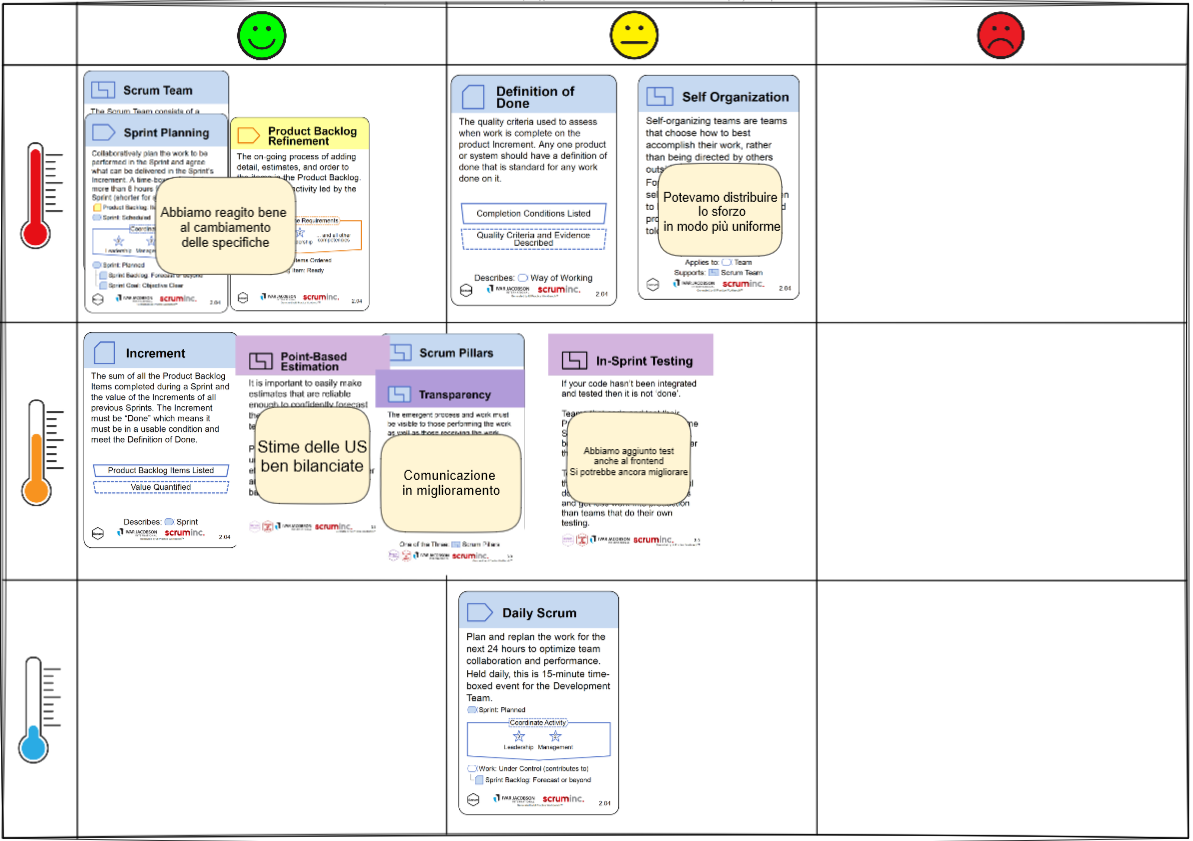
\includegraphics[width=15cm]{./img/sprint4/retrospettiva.png}
    \caption{Retrospettiva del 02/12/2022}
\end{figure}
\newpage

%%%

\newpage
\section{Descrizione del processo}

\subsection{Flusso di lavoro}
I ruoli di ciascun componente del gruppo nel processo di sviluppo sono stati i 
seguenti\footnote{Ad eccezione dello sprint 3 durante il quale è stato sperimentato l'inversione dei ruoli del team di sviluppo}:
\begin{center}
    \begin{tabular}{ | m{4cm} | m{10cm} | }
        \hline
        {\textbf{Membro}} & {\textbf{Ruoli}} \\
        \hline
        \makecell[cl]{Cheikh Ibrahim Zaid\\{\footnotesize PO Operativo}} & Sviluppo backend. Testing e quality assurance. \\ 
        \hline
        \makecell[cl]{Lee Qun Hao Henry\\{\footnotesize Developer}} & Sviluppo frontend. \\ 
        \hline
        \makecell[cl]{Paris Manuel\\{\footnotesize Developer}} & Sviluppo backend. \\ 
        \hline
        \makecell[cl]{Xia Tian Cheng\\{\footnotesize Scrum master}} & Sviluppo fullstack. Sistemista e CI/CD. \\ 
        \hline
    \end{tabular}
\end{center}

\subsubsection{Git}
L'organizzazione del repository git segue la metodologia \textit{gitflow} con un branch principale (\texttt{main}) che dopo ogni sprint viene allineato
con il branch di sviluppo (\texttt{dev}).\\
Più nello specifico, il flusso del lavoro ha seguito il seguente schema:
\begin{center}
\begin{tikzpicture}[auto, thick,
        node distance = 1cm and 1cm,
        pipestep/.style = {draw, align=center, minimum width=2cm, minimum height=1cm, rounded corners},
    ]
    \node[pipestep]                                     (taiga) {Selezione\\task su Taiga};
    \node[pipestep, right=of taiga]                     (git_branch) {Sviluppo su\\branch separato};
    \node[pipestep, right=of git_branch]                (mr) {Creazione\\merge request};
    \node[pipestep, below=of mr]                        (mr_approval1) {Approvazione\\tecnica};
    \node[pipestep, right=of mr_approval1]              (mr_approval2) {Approvazione\\del PO};
    \coordinate[right=of mr, xshift=0.8cm]              (padding);
    \node[pipestep, right=of padding]                   (merge) {Merge nel\\branch \texttt{dev}};
    \node[pipestep, below=of merge, yshift=-2cm]        (prod) {Merge nel\\branch \texttt{main}};
    %
    \draw[-stealth']  (taiga) -- (git_branch) node[midway, anchor=east] {};
    \draw[-stealth']  (git_branch) -- (mr) node[midway, anchor=east] {};
    \draw[-stealth']  (mr) -- (mr_approval1) node[midway, anchor=east] {};
    \draw[-stealth']  (mr_approval1) -- (mr_approval2) node[midway, anchor=east] {};
    \draw[-stealth']  (mr_approval2) -- (merge) node[midway, anchor=east] {};
    \draw[dashed,->]  (merge) -- (prod) node[midway, anchor=west, text width=1.5cm] {Termine sprint};
    % 
\end{tikzpicture}
\end{center}

\subsubsection{Bug tracking}
Per il tracciamento di problemi e bug sono stati usati gli strumenti disponibili in Gitlab e Taiga.
In particolare è stato utilizzato la funzionalità \textit{Issues} di Gitlab per creare e segnalare bug. 
Contemporaneamente è stato impostato Taiga in modo tale che venga integrato con Gitlab.\\
In questo modo sono visibile su entrambi gli strumenti le segnalazioni e il loro stato, permettendo una migliore pianificazione in fase di sprint planning e
una maggiore organizzazione durante lo sprint.

\subsubsection{Daily scrum}
Data l'impossibilità di effettuare incontri quotidiani, i daily scrum sono stati realizzati con cadenza più irregolare, tenendo una riunione almeno una volta a settimana
per allineare il team alla situazione del progetto (\textit{Weekly scrum}).\\
In aggiunta, con l'obiettivo sopperire alla mancanza di incontri giornalieri, sono stati effettuati dei \textit{daily scrum virtuali} su Mattermost.
Nello specifico, quando un componente decide di lavorare in una giornata, scrive un messaggio contenente la struttura di un daily scrum (ciò che svolgerà, ciò che ha svolto l'ultima volta ed eventuali problemi)
in modo tale da informare il team dell'avanzamento dei lavori.

\subsubsection{Monitoraggio delle ore di lavoro}
Per il tracciamento delle ore di lavoro è stata adottata una soluzione "manuale".
Ogni componente del gruppo è responsabile del monitoraggio delle proprie ore che compila in un file \texttt{json} presente in un repository su Gitlab \cite{timetracker_git}.\\
È inoltre presente una webapp \cite{timetracker} che elabora le informazioni inserite e si interfaccia con le API di Taiga, 
producendo una sintesi dei dati assieme a qualche statistica. 


\subsection{Team building}
\subsubsection{Scrumble}
La partita a Scrumble è stata giocata allo sprint 0, durante la fase preparatoria del progetto.\\
Lo scopo della sessione di team building era quella di prendere maggiore confidenza con la metodologia Scrum e 
confermare i ruoli all'interno del gruppo (Autovalutazione \cite{gqm_scrumble}).

\subsubsection{Escape the Boom}
La partita a Scrumble è stata giocata allo sprint 1.\\
L'obiettivo era quello di rafforzare la comunicazione nel team, che, come segnalato dal team alla retrospettiva (\fref{sprint1_retrospettiva}),
era carente e poco significativa (Autovalutazione \cite{gqm_escapetheboom}).


\subsection{Gitinspector}
I risultati di Gitinspector sono disponibili nel repository Gitlab \cite{gitinspector}. 
Per un'analisi più gradulare, sono state fatte le seguenti scansioni:
\begin{itemize}
    \item Complessiva su tutti i file
    \item Solo sui file che implementano funzionalità (quindi escludendo i test)
    \item Solo sui file contenenti test
\end{itemize}

Oltre a considerare come metriche la quantità di commit e il numero di righe inserite che possono variare dal metodo di lavoro del singolo,
risulta interessante analizzare il contributo di ciascun membro alle feature del prodotto.\\
È infatti possibile individuare le feature a cui ciascun componente del gruppo ha maggiormente contribuito:
\begin{center}
    \begin{tabular}{ | m{3cm} | m{11.5cm} | }
        \hline
        {\textbf{Membro}} & {\textbf{Funzionalità}} \\
        \hline
        \makecell[cl]{Cheikh Ibrahim\\Zaid} & 
        \makecell[cl]{%
            \begin{minipage}{\linewidth}
                \vspace*{0.15em}
                \begin{itemize}[leftmargin=1em]
                    \setlength\itemsep{-0.3em}
                    \item API per la ricerca di tweet per keyword
                    \item Modulo per la ricerca di un numero arbitrario di tweet
                    \item Componente con word cloud per i tweet
                    \item API per la parola vincente dei giochi televisivi
                    \item API per il \textit{Fantacitorio}
                \end{itemize}
            \end{minipage}
        } \\

        \hline

        \makecell[cl]{Lee\\Qun Hao Henry} & 
        \makecell[cl]{%
            \begin{minipage}{\linewidth}
                \vspace*{0.15em}
                \begin{itemize}[leftmargin=1em]
                    \setlength\itemsep{-0.3em}
                    \item Pagina di ricerca, visualizzazione e analisi dei tweet
                    \item Componente con mappa per la geolocalizzazione dei tweet
                    \item Componente con grafico a barre per la frequenza dei tweet
                    \item API per la raccolta dei tentativi degli utenti per i giochi televisivi
                    \item Pagina per il \textit{Fantacitorio}
                \end{itemize}
            \end{minipage}
        } \\

        \hline

        \makecell[cl]{Paris\\Manuel} & 
        \makecell[cl]{%
            \begin{minipage}{\linewidth}
                \vspace*{0.15em}
                \begin{itemize}[leftmargin=1em]
                    \setlength\itemsep{-0.3em}
                    \item API per la ricerca di tweet per nome utente
                    \item Modulo per la ricerca dei tweet per intervallo temporale
                    \item Componente con grafico a torta per il sentimento dei tweet
                    \item Pagina per i giochi televisivi
                    \item API per il \textit{Fantacitorio}
                \end{itemize}
            \end{minipage}
        } \\

        \hline

        \makecell[cl]{Xia\\Tian Cheng} & 
        \makecell[cl]{%
            \begin{minipage}{\linewidth}
                \vspace*{0.15em}
                \begin{itemize}[leftmargin=1em]
                    \setlength\itemsep{-0.3em}
                    \item API per l'analisi di tweet
                    \item Socket per la raccolta di tweet in tempo reale
                    \item Pagina di ricerca, visualizzazione e analisi dei tweet
                    \item Socket e pagina per lo scacchi
                    \item API per il \textit{Fantacitorio}
                \end{itemize}
            \end{minipage}
        } \\

        \hline
    \end{tabular}
\end{center}

È anche interessante analizzare l'andamento del numero di commit giornalieri nel tempo.
In particolare, se partizionata in base agli sprint, è possibile osservare alcuni comportamenti già evidenziati nella descrizione degli sprint (\fref{sprint_description}).
\begin{figure}[H]
    \centering
    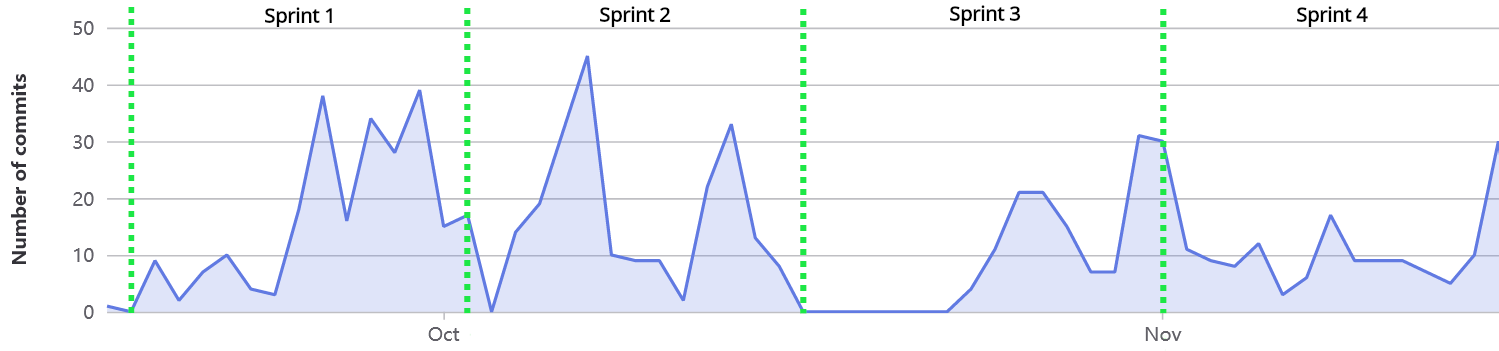
\includegraphics[width=15cm]{./img/git/commit.png}
    \caption{Andamento del numero di commit giornalieri, suddivisi per sprint}
\end{figure}


\subsection{Deployment}


\begin{center}
\begin{tikzpicture}[auto, thick,
        node distance = 1cm and 1 cm,
        pipestep/.style = {draw, align=center, minimum width=2.5cm, minimum height=1cm, rounded corners},
    ]
    \node[pipestep]                                     (gitlab) {
\includegraphics[width=1cm]{./img/icons/firefox.png}\\\textit{Push} su Gitlab};
    \node[pipestep, below=of gitlab]                    (jenkins) {
\includegraphics[width=1cm]{./img/icons/jenkins.png}\\Avvio pipeline\\Jenkins};
    \node[pipestep, right=of jenkins]                   (testing) {
\includegraphics[width=1cm]{./img/icons/jest.png}\\Testing};
    \coordinate[right=of testing, xshift=3cm]           (padding);
    \node[pipestep, above=of padding, yshift=0.5cm]     (deploy_prod) {
\includegraphics[width=1cm]{./img/icons/docker.png}\\Deploy produzione};
    \node[pipestep, below=of padding, yshift=-0.5cm]    (sonarqube) {
\includegraphics[width=1cm]{./img/icons/sonarqube.png}\\Sonarqube};
    \node[pipestep, right=of sonarqube]                 (deploy_dev) {
\includegraphics[width=1cm]{./img/icons/docker.png}\\Deploy\\ambiente di test};
    \node[pipestep, below=of testing]                   (mattermost) {
\includegraphics[width=1cm]{./img/icons/mattermost.png}\\Segnalazione su\\Mattermost};
    %
    \draw[-stealth']  (gitlab) -- (jenkins) node[midway, anchor=east, xshift=0.9cm, yshift=0.1cm, fill=white] {Webhook};
    \draw[-stealth']  (jenkins) -- (testing) node[midway, anchor=east] {};
    \draw[-stealth']  (testing.east) -- (deploy_prod.west) node[midway, anchor=east, xshift=1.6cm, yshift=-0.1cm, fill=white] {Branch \texttt{main}};
    \draw[-stealth']  (testing.east) -- (sonarqube.west) node[midway, anchor=east, xshift=1.2cm, yshift=0.1cm, fill=white] {Branch \texttt{dev}};
    \draw[-stealth']  (sonarqube) -- (deploy_dev) node[midway] {};
    \draw[-stealth']  (testing) -- (mattermost) node[midway, anchor=east, xshift=1.1cm, yshift=0.1cm, fill=white] {Fallimento};
    % 
\end{tikzpicture}
\end{center}


\newpage
\section{Artefatti}
L'accesso alle componenti dell'ambiente di sviluppo CAS avviene tramite \texttt{SSO Gitlab}.
\nocite{*}
\bibliographystyle{plain}
\bibliography{references}

\end{document}

